\begin{figure}[hbt]
    \centering
    \begin{subfigure}{.3\linewidth}
        \centering

        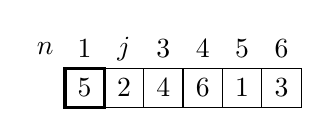
\begin{tikzpicture}
            \draw [very thick] (0.0, 0.0) rectangle (0.5, 0.5) node[midway]{5};
            \draw [] (0.5, 0.0) rectangle (1.0, 0.5) node[midway]{2};
            \draw [] (1.0, 0.0) rectangle (1.5, 0.5) node[midway]{4};
            \draw [] (1.5, 0.0) rectangle (2.0, 0.5) node[midway]{6};
            \draw [] (2.0, 0.0) rectangle (2.5, 0.5) node[midway]{1};
            \draw [] (2.5, 0.0) rectangle (3.0, 0.5) node[midway]{3};
            
            \path   node at (-0.25, 0.75) [] {$n$}
                    node at (0.25, 0.75) [] {1}
                    node at (0.75, 0.75) [] {$j$}
                    node at (1.25, 0.75) [] {3}
                    node at (1.75, 0.75) [] {4}
                    node at (2.25, 0.75) [] {5}
                    node at (2.75, 0.75) [] {6};
        \end{tikzpicture}

        \caption{\label{fig:insertions-example-begin}}
    \end{subfigure}
    \hfill
    \begin{subfigure}{.3\linewidth}
        \centering
        
        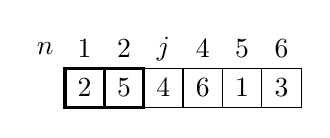
\begin{tikzpicture}
            \draw [very thick] (0.0, 0.0) rectangle (0.5, 0.5) node[midway]{2};
            \draw [very thick] (0.5, 0.0) rectangle (1.0, 0.5) node[midway]{5};
            \draw [] (1.0, 0.0) rectangle (1.5, 0.5) node[midway]{4};
            \draw [] (1.5, 0.0) rectangle (2.0, 0.5) node[midway]{6};
            \draw [] (2.0, 0.0) rectangle (2.5, 0.5) node[midway]{1};
            \draw [] (2.5, 0.0) rectangle (3.0, 0.5) node[midway]{3};
            
            \path   node at (-0.25, 0.75) [] {$n$}
                    node at (0.25, 0.75) [] {1}
                    node at (0.75, 0.75) [] {2}
                    node at (1.25, 0.75) [] {$j$}
                    node at (1.75, 0.75) [] {4}
                    node at (2.25, 0.75) [] {5}
                    node at (2.75, 0.75) [] {6};
        \end{tikzpicture}
        
        \caption{}
    \end{subfigure}
    \hfill
    \begin{subfigure}{.3\linewidth}
        \centering
        
        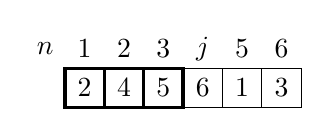
\begin{tikzpicture}
            \draw [very thick] (0.0, 0.0) rectangle (0.5, 0.5) node[midway]{2};
            \draw [very thick] (0.5, 0.0) rectangle (1.0, 0.5) node[midway]{4};
            \draw [very thick] (1.0, 0.0) rectangle (1.5, 0.5) node[midway]{5};
            \draw [] (1.5, 0.0) rectangle (2.0, 0.5) node[midway]{6};
            \draw [] (2.0, 0.0) rectangle (2.5, 0.5) node[midway]{1};
            \draw [] (2.5, 0.0) rectangle (3.0, 0.5) node[midway]{3};
            
            \path   node at (-0.25, 0.75) [] {$n$}
                    node at (0.25, 0.75) [] {1}
                    node at (0.75, 0.75) [] {2}
                    node at (1.25, 0.75) [] {3}
                    node at (1.75, 0.75) [] {$j$}
                    node at (2.25, 0.75) [] {5}
                    node at (2.75, 0.75) [] {6};
        \end{tikzpicture}

        \caption{}
    \end{subfigure}

    \bigskip
    \begin{subfigure}{.3\linewidth}
        \centering
        
        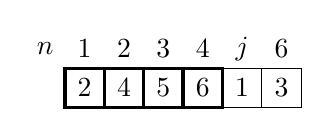
\begin{tikzpicture}
            \draw [very thick] (0.0, 0.0) rectangle (0.5, 0.5) node[midway]{2};
            \draw [very thick] (0.5, 0.0) rectangle (1.0, 0.5) node[midway]{4};
            \draw [very thick] (1.0, 0.0) rectangle (1.5, 0.5) node[midway]{5};
            \draw [very thick] (1.5, 0.0) rectangle (2.0, 0.5) node[midway]{6};
            \draw [] (2.0, 0.0) rectangle (2.5, 0.5) node[midway]{1};
            \draw [] (2.5, 0.0) rectangle (3.0, 0.5) node[midway]{3};
            
            \path   node at (-0.25, 0.75) [] {$n$}
                    node at (0.25, 0.75) [] {1}
                    node at (0.75, 0.75) [] {2}
                    node at (1.25, 0.75) [] {3}
                    node at (1.75, 0.75) [] {4}
                    node at (2.25, 0.75) [] {$j$}
                    node at (2.75, 0.75) [] {6};
        \end{tikzpicture}
        
        \caption{}
    \end{subfigure}
    \hfill
    \begin{subfigure}{.3\linewidth}
        \centering
        
        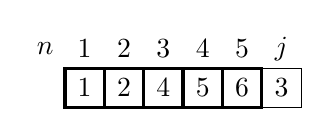
\begin{tikzpicture}
            \draw [very thick] (0.0, 0.0) rectangle (0.5, 0.5) node[midway]{1};
            \draw [very thick] (0.5, 0.0) rectangle (1.0, 0.5) node[midway]{2};
            \draw [very thick] (1.0, 0.0) rectangle (1.5, 0.5) node[midway]{4};
            \draw [very thick] (1.5, 0.0) rectangle (2.0, 0.5) node[midway]{5};
            \draw [very thick] (2.0, 0.0) rectangle (2.5, 0.5) node[midway]{6};
            \draw [] (2.5, 0.0) rectangle (3.0, 0.5) node[midway]{3};

            \path   node at (-0.25, 0.75) [] {$n$}
                    node at (0.25, 0.75) [] {1}
                    node at (0.75, 0.75) [] {2}
                    node at (1.25, 0.75) [] {3}
                    node at (1.75, 0.75) [] {4}
                    node at (2.25, 0.75) [] {5}
                    node at (2.75, 0.75) [] {$j$};
        \end{tikzpicture}

        \caption{\label{fig:insertions-example-end}}
    \end{subfigure}
    \hfill
    \begin{subfigure}{.3\linewidth}
        \centering
        
        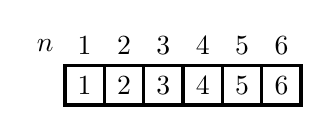
\begin{tikzpicture}
            \draw [very thick] (0.0, 0.0) rectangle (0.5, 0.5) node[midway]{1};
            \draw [very thick] (0.5, 0.0) rectangle (1.0, 0.5) node[midway]{2};
            \draw [very thick] (1.0, 0.0) rectangle (1.5, 0.5) node[midway]{3};
            \draw [very thick] (1.5, 0.0) rectangle (2.0, 0.5) node[midway]{4};
            \draw [very thick] (2.0, 0.0) rectangle (2.5, 0.5) node[midway]{5};
            \draw [very thick] (2.5, 0.0) rectangle (3.0, 0.5) node[midway]{6};
            
            \path   node at (-0.25, 0.75) [] {$n$}
                    node at (0.25, 0.75) [] {1}
                    node at (0.75, 0.75) [] {2}
                    node at (1.25, 0.75) [] {3}
                    node at (1.75, 0.75) [] {4}
                    node at (2.25, 0.75) [] {5}
                    node at (2.75, 0.75) [] {6};
        \end{tikzpicture}
        \caption{\label{fig:insertions-example-final}}
    \end{subfigure}
    % Underfull hbox because of the first line
    \caption{Illustration des Arrays $A = \{5, 2, 4, 6, 1, 3\}$ während es von $\proc{Insertion-Sort}(A)$ bearbeitet wird. Über einem Rechteck steht sein Index in $A$, in den Rechtecken steht der jeweilige Wert von $A$ an diesem Index. Fett gedruckte Rechtecke sind Teil des bereits sortierten Subarrays $A[1 \twodots j - 1]$. \subref{fig:insertions-example-begin} bis \subref{fig:insertions-example-end} zeigen die fünf Iterationen der $\For$-Schleife auf Zeilen \ref{ln:insertions-for-begin}--\ref{ln:insertions-for-end} beginnend mit $j = 2$ bis $j = \attrib{A}{length}$ beziehungsweise $j = 6$. Das Element $A[j]$ ist mit einem Obenstehendem $j$ gekennzeichnet, in der jeweils nächsten Iteration wurde es dann bereits an seine korrekte Position im sortierten Subarray $A[1 \twodots j - 1]$ bewegt. \subref{fig:insertions-example-final} zeigt das sortierte Array. Abbildungen \subref{fig:insertions-example-begin}--\subref{fig:insertions-example-end} sind maßgeblich inspiriert von \cite[18]{clrs2001}, Figure 2.2.}
    \label{fig:insertions-example}
\end{figure}
